%\documentclass{beamer}
%
%\usepackage{pgfpages} %This is needed for notes presentation!
%%\setbeameroption{}
%
%\usepackage{enumerate, amsmath, amssymb,amsthm, amstext,color}
%\usepackage[ngerman]{babel}
%\usepackage[utf8]{inputenc}   
%\usepackage{dsfont}
%\usepackage{geometry}
%\usepackage{fancyhdr}
%\usepackage{tikz}
%\usetikzlibrary{plotmarks}
%\usetikzlibrary{arrows, positioning}
%
%\usepackage{float}
%\usepackage{color}
%\usepackage{hyperref}
%% \usepackage{algorithmicx}
%% \usepackage{algpseudocode}
%\usepackage{fancybox}
%\usepackage{float}
%\usepackage{sidecap}
%\usepackage[ngerman]{babel}
%
%
%\newcommand{\lk}{\left}
%\newcommand{\rk}{\right}
%\newcommand{\rel}{\sqsubseteq}
%\newcommand{\rhn}{\mathds{R}^n}
% 
%  \usetheme{Berlin}
%%\usetheme{
%%	AnnArbor | Antibes | Bergen |
%%	Berkeley | Berlin | Boadilla |
%%	boxes | CambridgeUS | Copenhagen |
%%	Darmstadt | default | Dresden |
%%	Frankfurt | Goettingen |Hannover |
%%	Ilmenau | JuanLesPins | Luebeck |
%%	Madrid | Malmoe | Marburg |
%%	Montpellier | PaloAlto | Pittsburgh |
%%	Rochester | Singapore | Szeged |
%%	Warsaw
%%}
%\usecolortheme{beaver}
%% \usecolortheme{
%% 	albatross | beaver | beetle |
%% 	crane | default | dolphin |
%% 	dove | fly | lily | orchid |
%% 	rose |seagull | seahorse |
%% 	sidebartab | structure |
%% 	whale | wolverine
%% }
%
%\useinnertheme{rounded}
%% \useinnertheme{
%% 	circles | default | inmargin |
%% 	rectangles | rounded
%% }
%
%\useoutertheme{infolines}
%% \useoutertheme{
%% 	default | infolines | miniframes |
%% 	shadow | sidebar | smoothbars |
%% 	smoothtree | split | tree
%% }
%
%\usefonttheme{default}
%% \usefonttheme{
%% 	default | professionalfonts | serif |
%% 	structurebold | structureitalicserif |
%% 	structuresmallcapsserif
%% }
%
%% Seitenzahlen
%\setbeamertemplate{footline}[frame number]
%
%\title{Mid-term presentation}
%\author{The Quadrocopters}
%\institute{Technische Universität München}
%\date{\today}
%% \titlegraphic{\pgfimage[width=1cm,height=1cm]{MA_Web}}
%%\logo{\pgfimage[width=1.2cm,height=1.2cm]{MA_Web}}
%
%
%%\AtBeginSection[]{
%%	\frame{
%%	\frametitle{\"Ubersicht}
%%	\tableofcontents[current, currentSection]}
%%
%%}
%
%\setcounter{MaxMatrixCols}{20}

%\begin{document}

\definecolor{green}{RGB}{0,190,0};
\definecolor{red}{RGB}{190,0,0};
\definecolor{blue}{RGB}{0,0,190};

\begin{frame}
\maketitle
\end{frame}

\begin{frame}
\tableofcontents
\end{frame}

\section{Realtime Optimization Approach}
\begin{frame}{Setting}

\begin{figure}
\begin{tikzpicture}[scale=1.2]

%Draw bounding box
\draw (-2.75,-1.75) rectangle (3.75,3.25);

%Draw time line
\draw[ thick, ->] (-2.5,0) -- (2,0) node[anchor=west] {time};
\foreach  \t in  {-2, -1, +1}
	\draw[thick]  (\t cm, 1pt)  -- (\t cm, -1pt) node[anchor=north] {$t_{k \t  }$ };
\draw[thick]  (0cm , 1pt)  -- (0 cm, -1pt) node[anchor=north] {$t_k$ };

%draw known controls
\draw<2-> (2,1) node[anchor=west] {control};
\draw<2->[->,green] (-2.5, 0.8) -- (-2,0.8) ;
\draw<2->[->,green] (-2, 1.2) -- (-1,1.2) ;
\draw<2->[->,green] (-1, 0.9) -- (0,0.9) ;
\draw<4->[->,red,thick] (0, 1.1) -- (1,1.1) ;

%Draw actual time
\draw[dashed] (-.8,3) -- (-.8,-1) node[anchor=north] {$t_{act}$};

%Draw exact states
\draw<2-> (2,2) node[anchor=west] {state};
\draw<2->[green, fill=green] (-2, 2.2) circle (1pt) node[anchor=north]{\footnotesize $x_{k-2}$};
\draw<2->[green, fill=green] (-1, 1.9) circle (1pt) node[anchor=north]{\footnotesize $x_{k-1}$};
\draw<3->[red, fill=red] (0,2.1) circle (1pt) node[anchor=north]{\footnotesize $x_{k}$};
\end{tikzpicture}
\end{figure}
$y, s, q$ erklären



\end{frame}

\begin{frame}{Minimization Problem}
\begin{block}{ }
\begin{align*}
  \min_{\begin{array}{c} s_{t},...,s_{N}\\ q_{t},...,q_{N-1} \end{array}} \sum_{i=t}^{N-1} F_{i}(s_{i},q_{i}) \ \  
  s.t. \ \left\lbrace \begin{array}{c}
  x_{t} - s_{t} = 0 \\
  h_i (s_i ,q_i ) - s_{i+1} = 0 \ \ \forall i = t, ... , N-1 \end{array} \right. 
\end{align*}
\end{block}
\begin{tabular}{l l}
  $F_i(s_i, q_i)$ &  discretized goal function \\
$x_t - s_t = 0$ & expected state should be the real state at time $t$ \\
$h_i (s_i ,q_i )$ & solution of the ODE at time $i$ \\
\end{tabular}
\end{frame}

\begin{frame}{The Lagrangian}
\begin{block}{ }
\begin{align*}
  L^{t}(y) = \sum_{i=t}^{N-1} F_{i}(s_{i},q_{i})
  + \lambda_{t}^{T}(x_{t} - s_{t})
  + \sum_{i=t}^{N-1} \lambda_{i+1}^{T} (h_i (s_i ,q_i ) - s_{i+1})
\end{align*}
\end{block}
\begin{center}
We are looking for $y^*$ satisfying the KKT conditions. \\

$\Rightarrow \nabla_{y} L^{t}(y^*)  = 0 $ 

\end{center}
\end{frame}

\begin{frame}{The SQP method}
How do we find $y^*$?
\begin{align*}
  y_{k+1} = y_{k} + \alpha_{k} \Delta y_{k}
\end{align*}
\begin{align*}
\Downarrow
\end{align*}
\begin{align*}
\min_{\Delta y} = \frac{1}{2} \Delta y^T A_k \Delta y + \nabla_y F(y_k)^T \Delta y
\end{align*}
\begin{align*}
\Downarrow
\end{align*}
\begin{align*}
A_{k} := \nabla^{2}_{y_k} L(y_k).
\end{align*}
  
\end{frame}

\begin{frame}{Newton-Raphson}
\begin{block}{}
\begin{gather*}
y_{t+1} = y_t + \Delta y_t \\
\nabla_{y_t} L^{t}(y_{t}) + J^{t}(y_{t}) \Delta y_{t} = 0
\end{gather*}
\end{block}
\begin{tabular}{l l}
  $J^t(y_t)$ & Approximated Hessian $\nabla^{2}_{y_t} L(y_t)$ \\
  $\alpha_t = 1$ & 
\end{tabular}
\end{frame}

\begin{frame}{Riccati Recursion}
This formulation still depends on $x_t$ ...
\begin{align*} 
  \scriptstyle{J^{t}(y^{t})} =
  \tiny{
	\begin{pmatrix}
		& -E  &     &     &     &     &     &     &     &     &     \\ \\
-E  & Q_t^{H} & M_t^{H} & A_t^{T} &  &    &     &     &     &     &     \\ \\
    & (M_t^{T})^{H} & R_t^{H} & B_t^{T} &   &    &    &    &    &   &     \\ \\
    & A_t & B_t &     & -E  &     &     &     &     &     &     \\ \\
    &  &  & -E  & Q_{t+1}^{H} & M_{t+1}^{H} & A_{t+1}^{T} &  &  &  &  \\ \\
    &  &  &     & (M_{t+1}^{T})^{H} & R_{t+1}^{H} & B_{t+1}^{T} &  &  &  &  \\ \\
    &  &  &     & A_{t+1} & B_{t+1} &    &    &     &     &     \\ \\
    &  &  &     &    &    &   & \ddots &     &     &     \\ \\
    &  &  &   &  &  & \ddots & Q_{N-1}^{H} & M_{N-1}^{H} & A_{N-1}^{T} &  \\ \\
    &  &  &   &  &  &    & (M_{N-1}^{T})^{H} & R_{N-1}^{H} & B_{N-1}^{T} &  \\ \\
    &  &  &   &  &  &    & A_{N-1}     & B_{N-1} &    & -E \\ \\
    &  &  &     &    &    &     &      &     & -E &  Q_N^{H} 
\end{pmatrix}
}
  \end{align*}

\end{frame}

\begin{frame}{Summary}
What happens in interval $ [ t_{k-1} , t_k ] $ ?
\begin{figure}
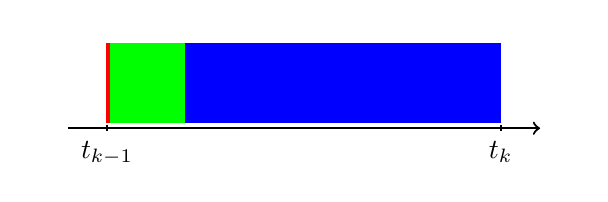
\begin{tikzpicture}
%Draw bounding box
\draw[white] (-1,-.5) rectangle (6,1.2);

%Draw time line
\draw[ thick, ->] (-.5,-2pt) -- (5.5,-2pt);

\draw[thick]  (5 cm, -1pt)  -- (5 cm, -3pt) node[anchor=north] {$t_{k }$ };
\draw[thick]  (0cm , -1pt)  -- (0 cm, -3pt) node[anchor=north] {$t_{k-1}$ };

%Solve for control in t_k-1
\draw<2->[red,fill=red] (0,0) rectangle (0.05, 1);
% Calculcate start value for t_k
\draw<3->[green, fill=green] (0.05,0) rectangle (1, 1);
%Prepare for t_k
\draw<4->[blue,fill=blue] (1,0) rectangle (5,1);
\end{tikzpicture}
\end{figure}

\begin{enumerate}
\item<2-> {\color{red} Calculate control $u_{k-1}$}
\item<3-> {\color{green} Calculate $y_k$ ( Riccati Part II)}
\item<4-> {\color{blue} Prepare $u_k$ (SQP \& Riccati Part I)} 
\end{enumerate}
\end{frame}

\begin{frame}{Finite Horizon}
how to choose $N$?
\begin{itemize}
\item $N=t_{end}$ problem gets smaller every time 
\item $N=t+n$ problem size is constant
\item .
\item .
\item .
\end{itemize}

\end{frame}
%\end{document}